% Created 2024-10-16 śro 21:35
% Intended LaTeX compiler: pdflatex
\documentclass[../../main.tex]{subfiles}

% \usepackage[a4paper, margin=3cm]{geometry}
% \usepackage{amssymb} // not working

\usepackage[T1]{fontenc}
\usepackage[utf8]{inputenc}
\usepackage{graphicx}
\usepackage{longtable}
\usepackage{wrapfig}
\usepackage{rotating}
\usepackage[normalem]{ulem}
\usepackage{amsmath}
\usepackage{capt-of}
\usepackage{hyperref}
\usepackage{siunitx}
\usepackage{float}
\usepackage[polish]{babel}

\graphicspath{{../}}
\author{Wojciech Paderewski}
\date{\today}
\title{LDO}
\hypersetup{
 pdfauthor={Wojciech Paderewski},
 pdftitle={LDO},
 pdfkeywords={},
 pdfsubject={},
 pdflang={Polish}}

\begin{document}

Moduł jest odpowiedzialny za sterowanie wyświetlaniem cyfr na lampach Nixie oraz załączanie lamp neonowych.
Sterowanie lampami i neonówkami odbywa się za pomocą rejestrów przesuwnych, które są sterowane przez mikrokontroler.
Natomiast kropki na lampach Nixie są sterowane za pośrednictwem tranzystorów.

\subsubsection{Dobór rejestrów}
Wybrano rejestry przesuwne HV firmy microchip o numerze HV5530, o nastepujacych parametrach \cite{st:rejestry}:
\begin{itemize}
    \item Rejestr 32 bitowy
    \item Maksymalne napięcie na wyjściu - \SI{315}{\volt}
    \item Maksymalna częstotliwość pracy - \SI{8}{\mega\hertz}
    \item napięcie zasilania - od \SI{10.8}{\volt} do \SI{13.6}{\volt}
    \item stan wysoki - $V_{cc} - \SI{2}{\volt}$ gdzie $V_{cc}$ to napięcie zasilania
\end{itemize}

\subsubsection{Sterowanie rejestrów}
Sterowanie rejestrem realizowane jest za pomocą nastepujacych pinów:
\begin{itemize}
    \item CLK - sterowanie zegarem rejestru
    \item LE - załadowanie danych do rejestru(Latch Enable)
    \item POL - ustawienie polaryzacji wyjścia
    \item DATA\_IN - wejście danych
    \item BL - wyjście blanking(ustawianie wszystkich wyjść na zadany stan logiczny)
    \item DATA\_OUT - wyjście danych dla następnego rejestru
\end{itemize}

Do sterowania wystarczą jedynie 3 linie CLK, LE, DATA\_IN, ponieważ BL i POL można ustawić na stałe.
Rejestry można połączyć ze sobą dzięki czemu wymagana jest tylko jedna linia danych.
Sterowanie wymaga użycia konwertera poziomów logicznych, ponieważ mikrokontroler pracuje na napięciu \SI{3.3}{\volt}, a rejestr operuje 
na napięciu około \SI{12}{\volt}.

Zastosowano konwerter poziomów logicznych CD40109B-Q1 firmy Texas Instruments \cite{st:konwerter}.
Konwerter jest 4 kanałowy, co pozwala na podłączenie 4 sygnałów, więc wybrano połaczenia
CLK, LE, DATA\_IN, BL. Konwerter pracuje w zakresie napięć od \SI{3}{\volt} do \SI{20}{\volt}, więc spełnia wymagania.

\subsubsection{Sterowanie kropkami dziesiętnymi}
Sterowanie kropkami dziesiętnymi odbywa się za pomocą tranzystorów HV firmy Diodes Industries o numerze DMN60H080DS, 
o nastepujacych parametrach \cite{st:rejestry}:
\begin{itemize}
    \item maksymalne napięcie dren-źródło - \SI{600}{\volt}
    \item maksymalny prąd drenu - \SI{80}{\milli\ampere}
    \item napięcie progowe - ok. \SI{2}{\volt}
\end{itemize}

\subsubsection{Dobór rezystorów}
Wartość rezystorów anodowych dla zastosowanych lamp zostały obliczone w rozdziale \ref{sec:nixie}.
Kropki wymagają mniejszego prądu, producent jednak nie podaje dokładnej wartości, więc przyjęto wartość \SI{51}{\kilo\ohm}.
Dobór rezystora zostanie oceniony empirycznie, podczas testowania gotowego układu.

Lampy neonowe mają zdecydowanie mniejszy prąd pracy oraz mniejsze napięcie pracy. W sklepie internetowym sprzedający deklarował nastepujace parametry:
\begin{itemize}
    \item wymagane napięcie - \SI{90}{\volt}
    \item prąd pracy - \SI{0.3}{\milli\ampere}
\end{itemize}

\begin{equation}
    R = \frac{U}{I} = \frac{\SI{220}{\volt} - \SI{90}{\volt}}{ \SI{0.3}{\milli\ampere}} \approx \SI{433}{\kilo\ohm}
\end{equation}

Rezystor potrzebny do zabezpieczenia lampy neonowej przy napięciu zasilania \SI{220}{\volt} powinien mieć wartość około \SI{433}{\kilo\ohm}.
Zdecydowano się na użycie rezystora o wartości \SI{390}{\kilo\ohm}, ze względu na dostępność w sklepie internetowym. 
Schemat elektryczny zaprojektowanego modułu przedstawiono na rysunku \ref{fig:nixie}.

\begin{figure}[H]
    \centering
    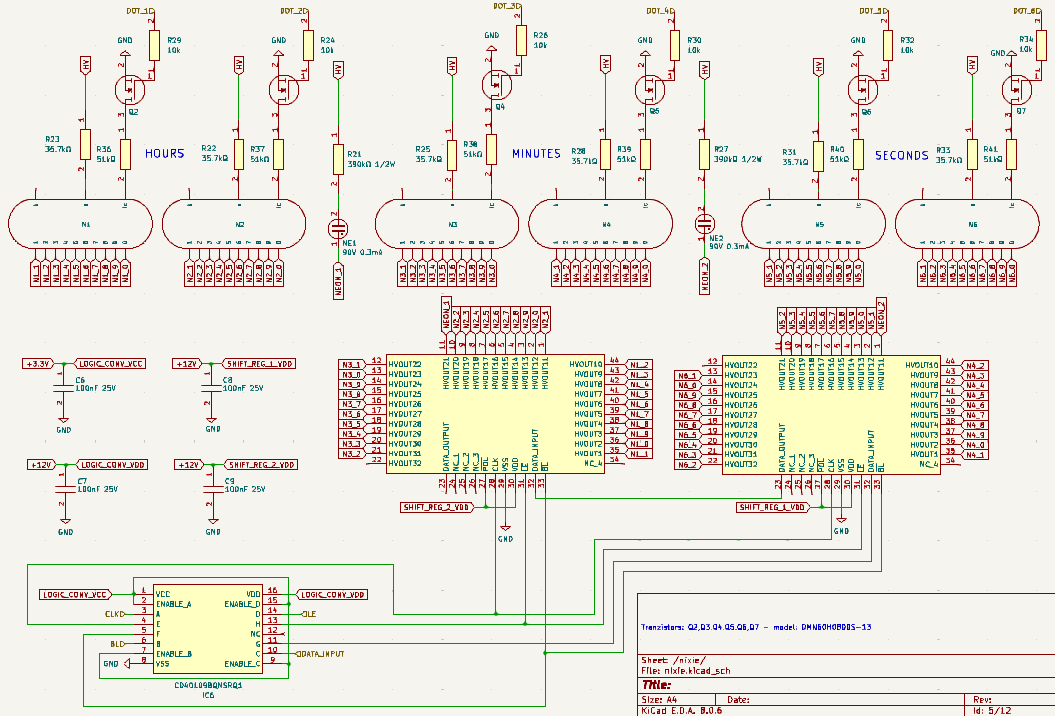
\includegraphics[width=0.95\textwidth]{nixie.png}
    \caption{Schemat elektryczny modułu sterowania lampami}
    \label{fig:nixie}
\end{figure}

\end{document}
